%LTeX: language=it
\subsection{UC 5 - Creazione evento} \label{sec:UC5}
    \begin{itemize}
        \item \textbf{Attore principale}: MUA;
        \item \textbf{Descrizione}: il MUA deve poter creare un evento nel sistema;
        \item \textbf{Precondizioni}: l’account che il MUA gestisce è registrato nel sistema, ha un connessione aperta con il sistema ed è autenticato;
        \item \textbf{Postcondizioni}: il MUA crea l'evento che viene salvato nel sistema;
        \item \textbf{Scenario principale}:
            \begin{enumerate}
                \item il MUA trasmette il titolo dell'evento (\hyperref[sec:UC5.1]{UC 5.1});
                \item il MUA trasmette la data di inizio dell'evento (\hyperref[sec:UC5.2]{UC 5.2});
                \item \item il MUA trasmette la data di fine dell'evento (\hyperref[sec:UC5.3]{UC 5.3});
                \item il MUA trasmette la durata dell'evento (\hyperref[sec:UC5.4]{UC 5.4});
                \item il sistema salva l'evento;
            \end{enumerate}
        \item \textbf{Inclusioni}: nessuna;
        \item \textbf{Generalizzazioni}: nessuna;
        \item \textbf{Estensioni}: 
        \begin{enumerate}[label=\alph*.]
            \item il sistema non riesce a creare l'evento perchè il titolo non è valido:
            \begin{enumerate}[label=\arabic*.]
                \item il sistema ritorna un errore al MUA di titolo evento non valido (\hyperref[sec:UC5.5]{UC 5.5}).
            \end{enumerate}
            \item il sistema non riesce a creare l'evento perchè la data di inizio dell'evento non è in un formato valido:
            \begin{enumerate}[label=\arabic*.]
                \item il sistema ritorna un errore al MUA di data non valida (\hyperref[sec:UC5.6]{UC 5.6}).
            \end{enumerate}
            \item il sistema non riesce a creare l'evento perchè la data di fine dell'evento non è in un formato valido:
            \begin{enumerate}[label=\arabic*.]
                \item il sistema ritorna un errore al MUA di data non valida (\hyperref[sec:UC5.6]{UC 5.6}).
            \end{enumerate}
            \item il sistema non riesce a creare l'evento perchè la durata dell'evento è inconsistente rispetto alla data di inizio e di fine:
            \begin{enumerate}[label=\arabic*.]
                \item il sistema ritorna un errore al MUA di durata inconsistente (\hyperref[sec:UC5.7]{UC 5.7}).
            \end{enumerate}
        \end{enumerate}
    \end{itemize}

\begin{figure}[H]
    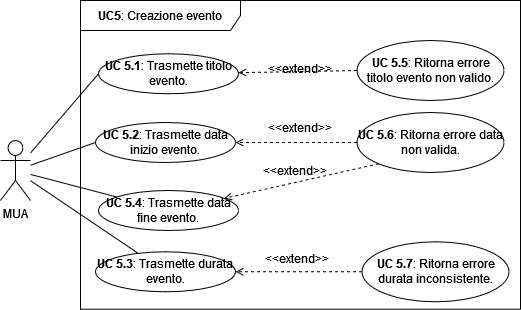
\includegraphics[width=0.85\textwidth]{sections/uc_imgs/UC05.png}
    \centering
    \caption{Diagramma sotto-casi UC 5}
\end{figure}

\subsubsection{UC 5.1 - Trasmette titolo evento} \label{sec:UC5.1}
    \begin{itemize}
        \item \textbf{Attore principale}: MUA;
        \item \textbf{Descrizione}: il MUA trasmette il titolo per creare l'evento al sistema;
        \item \textbf{Precondizioni}: il MUA sta usando la funzionalità di creazione di un evento;
        \item \textbf{Postcondizioni}: il sistema conosce il titolo dell'evento;
        \item \textbf{Scenario principale}:
            \begin{enumerate}
                \item il MUA invia il titolo per creare l'evento al sistema;
                \item il sistema controlla che le informazioni ricevute rispettino il seguente requisito minimo:
                    \begin{itemize}
                        \item il titolo dell'evento non è una stringa vuota;
                    \end{itemize}
            \end{enumerate}
        \item \textbf{Inclusioni}: nessuna;
        \item \textbf{Generalizzazioni}: nessuna;
        \item \textbf{Estensioni}:
            \begin{enumerate}[label=\alph*.]
                \item il sistema non riesce a creare l'evento perché il titolo fornito non è valido:
                \begin{enumerate}[label=\arabic*.]
                    \item il sistema ritorna un errore al MUA di titolo evento non valido (\hyperref[sec:UC5.5]{UC 5.5}).
                \end{enumerate}
            \end{enumerate}
    \end{itemize}



    \subsubsection{UC 5.2 - Trasmette data inizio evento} \label{sec:UC5.2}
    \begin{itemize}
        \item \textbf{Attore principale}: MUA;
        \item \textbf{Descrizione}: il MUA trasmette la data di inizio dell'evento per creare l'evento al sistema;
        \item \textbf{Precondizioni}: il MUA sta usando la funzionalità di creazione di un evento;
        \item \textbf{Postcondizioni}: il sistema conosce la data di inizio dell'evento;
        \item \textbf{Scenario principale}:
            \begin{enumerate}
                \item il MUA invia la data di inizio dell'evento per creare l'evento al sistema;
                \item il sistema controlla che le informazioni ricevute rispettino il seguente requisito minimo:
                    \begin{itemize}
                        \item la data di inizio dell'evento è in un formato corretto;
                    \end{itemize}
            \end{enumerate}
        \item \textbf{Inclusioni}: nessuna;
        \item \textbf{Generalizzazioni}: nessuna;
        \item \textbf{Estensioni}:
            \begin{enumerate}[label=\alph*.]
                \item il sistema non riesce a creare l'evento perché la data di inizio dell'evento fornita non è in un formato corretto:
                \begin{enumerate}[label=\arabic*.]
                    \item il sistema ritorna un errore al MUA di data evento non valida (\hyperref[sec:UC5.6]{UC 5.6}).
                \end{enumerate}
            \end{enumerate}
    \end{itemize}


    \subsubsection{UC 5.3 - Trasmette data fine evento} \label{sec:UC5.3}
    \begin{itemize}
        \item \textbf{Attore principale}: MUA;
        \item \textbf{Descrizione}: il MUA trasmette la data di fine dell'evento per creare l'evento al sistema;
        \item \textbf{Precondizioni}: il MUA sta usando la funzionalità di creazione di un evento;
        \item \textbf{Postcondizioni}: il sistema conosce la data di fine dell'evento;
        \item \textbf{Scenario principale}:
            \begin{enumerate}
                \item il MUA invia la data di fine dell'evento per creare l'evento al sistema;
                \item il sistema controlla che le informazioni ricevute rispettino il seguente requisito minimo:
                    \begin{itemize}
                        \item la data di fine dell'evento è in un formato corretto;
                    \end{itemize}
            \end{enumerate}
        \item \textbf{Inclusioni}: nessuna;
        \item \textbf{Generalizzazioni}: nessuna;
        \item \textbf{Estensioni}:
            \begin{enumerate}[label=\alph*.]
                \item il sistema non riesce a creare l'evento perché la data di fine dell'evento fornita non è in un formato corretto:
                \begin{enumerate}[label=\arabic*.]
                    \item il sistema ritorna un errore al MUA di data evento non valida (\hyperref[sec:UC5.6]{UC 5.6}).
                \end{enumerate}
            \end{enumerate}
    \end{itemize}

    \subsubsection{UC 5.4 - Trasmette durata evento} \label{sec:UC5.4}
    \begin{itemize}
        \item \textbf{Attore principale}: MUA;
        \item \textbf{Descrizione}: il MUA trasmette la durata per creare l'evento al sistema;
        \item \textbf{Precondizioni}: il MUA sta usando la funzionalità di creazione di un evento;
        \item \textbf{Postcondizioni}: il sistema conosce la durata dell'evento;
        \item \textbf{Scenario principale}:
            \begin{enumerate}
                \item il MUA invia la durata per creare l'evento al sistema;
                \item il sistema controlla che le informazioni ricevute rispettino il seguente requisito minimo:
                    \begin{itemize}
                        \item la durata dell'evento deve essere consistente con la data di inizio e la data di fine;
                    \end{itemize}
            \end{enumerate}
        \item \textbf{Inclusioni}: nessuna;
        \item \textbf{Generalizzazioni}: nessuna;
        \item \textbf{Estensioni}:
            \begin{enumerate}[label=\alph*.]
                \item il sistema non riesce a creare l'evento perché la durata fornita non è valido:
                \begin{enumerate}[label=\arabic*.]
                    \item il sistema ritorna un errore al MUA di durata inconsistente (\hyperref[sec:UC5.7]{UC 5.7}).
                \end{enumerate}
            \end{enumerate}
    \end{itemize}


    \subsubsection{UC 5.5 - Ritorna errore titolo evento non valido} \label{sec:UC5.5}
    \begin{itemize}
        \item \textbf{Attore principale}: MUA;
        \item \textbf{Descrizione}: il sistema non riesce a salvare l'evento perché il titolo dell'evento non rispetta i requisiti;
        \item \textbf{Precondizioni}: il MUA ha inviato il titolo dell'evento;
        \item \textbf{Postcondizioni}: il sistema non salva il nuovo evento, il MUA è stato notificato dell'errore;
        \item \textbf{Scenario principale}:
            \begin{enumerate}
                \item il sistema controlla la sintassi del titolo dell'evento e trova un errore;
                \item il sistema non salva l'evento e notifica il MUA dell'errore;
            \end{enumerate}
        \item \textbf{Inclusioni}: nessuna;
        \item \textbf{Generalizzazioni}: nessuna;
        \item \textbf{Estensioni}: nessuna.
    \end{itemize}


    \subsubsection{UC 5.6 - Ritorna errore data non valida} \label{sec:UC5.6}
    \begin{itemize}
        \item \textbf{Attore principale}: MUA;
        \item \textbf{Descrizione}: il sistema non riesce a salvare l'evento perché la data non rispetta i requisiti;
        \item \textbf{Precondizioni}: il MUA ha inviato il titolo dell'evento;
        \item \textbf{Postcondizioni}: il sistema non salva il nuovo evento, il MUA è stato notificato dell'errore;
        \item \textbf{Scenario principale}:
            \begin{enumerate}
                \item il sistema controlla il formato della data dell'evento e trova un errore;
                \item il sistema non salva l'evento e notifica il MUA dell'errore;
            \end{enumerate}
        \item \textbf{Inclusioni}: nessuna;
        \item \textbf{Generalizzazioni}: nessuna;
        \item \textbf{Estensioni}: nessuna.
    \end{itemize}

    \subsubsection{UC 5.7 - Ritorna errore durata inconsistente} \label{sec:UC5.7}
    \begin{itemize}
        \item \textbf{Attore principale}: MUA;
        \item \textbf{Descrizione}: il sistema non riesce a salvare l'evento perché la durata non rispetta i requisiti;
        \item \textbf{Precondizioni}: il MUA ha inviato la durata dell'evento;
        \item \textbf{Postcondizioni}: il sistema non salva il nuovo evento, il MUA è stato notificato dell'errore;
        \item \textbf{Scenario principale}:
            \begin{enumerate}
                \item il sistema controlla ila consistenza della durata e trova un errore;
                \item il sistema non salva l'evento e notifica il MUA dell'errore;
            \end{enumerate}
        \item \textbf{Inclusioni}: nessuna;
        \item \textbf{Generalizzazioni}: nessuna;
        \item \textbf{Estensioni}: nessuna.
    \end{itemize}